\documentclass[11pt]{article}
\usepackage[margin=2.5cm]{geometry}
\usepackage{graphicx}
\usepackage{booktabs}
\usepackage{amsmath}
\usepackage{float}
\usepackage{hyperref}
\graphicspath{{figures/}}

\title{Active Learning for Learning to Defer\\\large Human Centric Artificial Intelligence Project 3}
\author{Mohamed Refaat\\Matriculation number: 670229}
\date{}


\begin{document}
\maketitle

\section{Introduction}
The goal of this project is to build a classification system that collaborates with a human expert. Given a news article from the AG News dataset (four classes: World, Sports, Business, Sci/Tech: 120{,}000 training and 7{,}600 test articles), the system can either predict the class itself or defer the decision to an expert. Since expert annotations are expensive, the central question is how to learn when deferral is beneficial while querying the expert as little as possible.

The report is structured as follows. Section~\ref{sec:baseline} describes the baseline classifier. Section~\ref{sec:expert} describes and analyzes the simulated expert. Section~\ref{sec:l2d} presents a learning to defer system trained with full access to expert predictions, which serves as an upper reference for the active learning setting. Section~\ref{sec:al} presents the main contribution: a controlled comparison of five query strategies for discovering the expert's competence, from which the final utility function is selected.

\section{Baseline Classifier}
\label{sec:baseline}
The baseline is a TF-IDF representation (50{,}000 features) combined with multinomial logistic regression ($C=1$, trained on all 120{,}000 labeled articles, \texttt{random\_state}=42). This choice is motivated by three considerations: it is a strong and standard approach for topic classification at this scale, it trains in minutes on a CPU, and it produces class probabilities that are later reused by the uncertainty based query strategies.

\begin{table}[H]
\centering
\begin{tabular}{lc}
\toprule
Metric & Accuracy \\
\midrule
Training accuracy & 94.62\% \\
Test accuracy & \textbf{91.89\%} \\
\bottomrule
\end{tabular}
\caption{Baseline classifier performance.}
\end{table}

The test accuracy of 91.89\% is the benchmark that the human AI team should match or surpass.

\section{Simulated Expert}
\label{sec:expert}
The simulated expert is designed with a Perfect knowledge in two categories: it answers World and Sports articles correctly, and answers uniformly at random over the four classes on Business and Sci/Tech articles. 

\begin{table}[H]
\centering
\begin{tabular}{lc}
\toprule
Category & Expert accuracy \\
\midrule
World & 100\% \\
Sports & 100\% \\
Business & $\approx$25\% \\
Sci/Tech & $\approx$25\% \\
\midrule
Overall & $\approx$62\% \\
\bottomrule
\end{tabular}
\caption{Simulated expert performance on the test set.}
\end{table}

The classifier on the category World reaches 90.53\% and on Sports 97.95\%, both below the expert. On Business and Sci/Tech the expert performs randomly. Used alone, the expert (62\%) is far worse than the classifier (91.89\%); its value can only be used through deferral.

\section{Learning to Defer with Full Expert Information}
\label{sec:l2d}
In this section the expert's predictions are assumed available for every training point. In addition to the classifier, a deferral model $r(x)$ is trained to decide, per input, whether the system predicts itself or defers; the final prediction is the expert's if $r(x)$ defers and the classifier's otherwise.

The deferral model is a logistic regression on the same TF-IDF features with balanced class weights, trained on binary labels indicating whether the article lies in the expert's competence region (World or Sports). An initial variant labeled a point ``defer'' only when the expert was correct \emph{and} the classifier wrong; this produced roughly 5\% positive labels and the resulting model collapsed to never deferring.

\begin{table}[H]
\centering
\begin{tabular}{lc}
\toprule
Metric & Value \\
\midrule
System accuracy & \textbf{93.04\%} \\
Deferral decision accuracy & 95.28\% \\
Deferral rate & 50.12\% \\
\midrule
Classifier alone & 91.89\% \\
Expert alone & $\approx$62\% \\
\bottomrule
\end{tabular}
\caption{learning to defer system with full expert information.}
\end{table}

\begin{table}[H]
\centering
\begin{tabular}{lcc}
\toprule
Category & System accuracy & Classifier alone \\
\midrule
World & 94.16\% & 90.53\% \\
Sports & 99.21\% & 97.95\% \\
Business & 88.00\% & 88.32\% \\
Sci/Tech & 90.79\% & 90.79\% \\
\bottomrule
\end{tabular}
\caption{Per class effect of deferral.}
\end{table}

The system beats both agents individually, deferring approximately the World/Sports half of the data to the expert and handling the rest itself. Evaluation covers not only accuracy, but also the quality of deferral. decisions.

\section{Active Learning for Expert Competence Discovery}
\label{sec:al}

\subsection{Problem setting}
From now on, no expert labels are available in advance. The system may query the expert on individual training points, at a cost. The objective is to train a predictor of whether the expert would answer a given input correctly, which would enable good deferral decisions with as few queries as possible.

\subsection{Candidate utility functions}
Five query strategies were implemented. Given classifier probabilities $p(x)$ over classes:
\begin{itemize}
\item \textbf{Random}: uniform sampling from the unqueried pool.
\item \textbf{Entropy}: query points maximizing $H(x) = -\sum_k p_k(x)\log p_k(x)$.
\item \textbf{Least confidence}: query points maximizing $1 - \max_k p_k(x)$.
\item \textbf{Margin}: query points minimizing the gap between the two highest class probabilities.
\item \textbf{Competence uncertainty}: query points where the current competence model is most uncertain, i.e. minimizing $|P_{\text{comp}}(\text{correct}\,|\,x) - 0.5|$. In the first round, before any competence model exists, it goes back to random sampling.
\end{itemize}

\subsection{Experimental protocol}
Each strategy runs for 10 rounds of 100 queries (1{,}000 expert queries total, under 1\% of the training pool). After each round, the competence model (logistic regression, balanced class weights) is retrained on all collected (input, expert correct) pairs, and the deferral system, defer where the competence model predicts the expert is correct, is evaluated on the test set. Every strategy is run with three random seeds (42--44); plots report mean $\pm$ standard deviation. Three metrics are tracked: system accuracy, coverage (fraction of inputs not deferred), and the competence model's balanced accuracy at predicting the expert's correctness on the test set. Three reference baselines are shown: classifier alone (91.89\%), expert alone ($\approx$62--63\%), and full information deferral ($\approx$94.7\%), which defers exactly on World/Sports and represents the ceiling any deferral policy can reach with this classifier and expert.

\subsection{Results}

\begin{figure}[H]
\centering
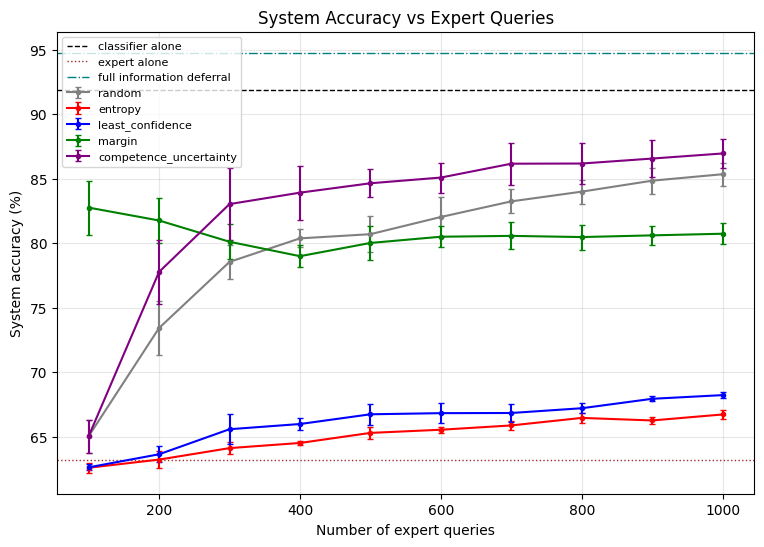
\includegraphics[width=0.85\textwidth]{al_accuracy.png}
\caption{System accuracy versus number of expert queries.}
\label{fig:acc}
\end{figure}

\begin{figure}[H]
\centering
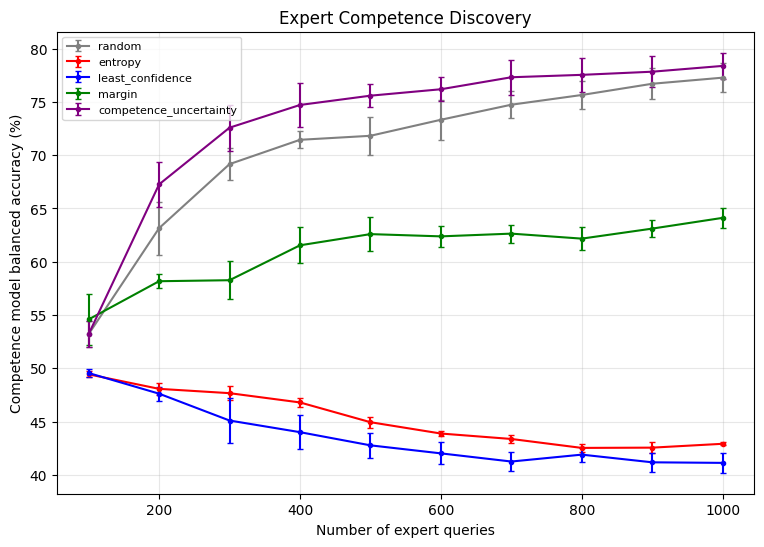
\includegraphics[width=0.85\textwidth]{al_competence.png}
\caption{Competence discovery: balanced accuracy of the competence model.}
\label{fig:comp}
\end{figure}

\begin{figure}[H]
\centering
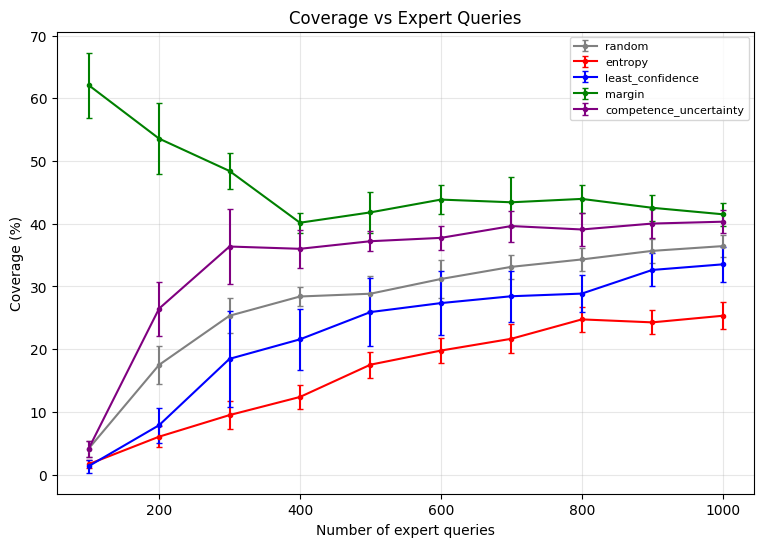
\includegraphics[width=0.85\textwidth]{al_coverage.png}
\caption{Coverage versus number of expert queries.}
\label{fig:cov}
\end{figure}

\begin{figure}[H]
\centering
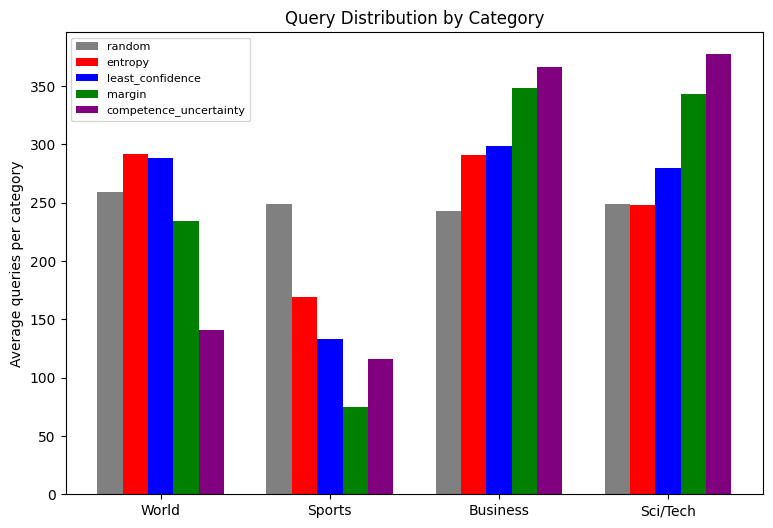
\includegraphics[width=0.85\textwidth]{al_distribution.png}
\caption{Distribution of expert queries across categories (average per seed).}
\label{fig:dist}
\end{figure}

\begin{table}[H]
\centering
\begin{tabular}{lccc}
\toprule
Strategy & System acc. & Coverage & Competence bal. acc. \\
\midrule
Competence uncertainty & \textbf{$\approx$87.0\%} & $\approx$40\% & \textbf{$\approx$78.5\%} \\
Random & $\approx$85.4\% & $\approx$36.5\% & $\approx$77.3\% \\
Margin & $\approx$80.7\% & $\approx$41.5\% & $\approx$64.1\% \\
Least confidence & $\approx$68.2\% & $\approx$33.7\% & $\approx$41.2\% \\
Entropy & $\approx$66.8\% & $\approx$25.4\% & $\approx$43.0\% \\
\bottomrule
\end{tabular}
\caption{Final values after 1{,}000 queries (mean over 3 seeds, read from the final round).}
\end{table}

\subsection{Analysis}
The classifier uncertainty utilities (entropy, least confidence) fail severely: their competence models end \emph{below} 50\% balanced accuracy, i.e.\ systematically wrong. The mechanism is that these strategies sample boundary and atypical articles. Consider a World article that the classifier confuses with Business: in feature space it resembles a Business article, yet the expert answers it correctly since it is truly World. Meanwhile genuine Business queries are answered randomly. The competence model therefore receives contradictory and, for typical articles, inverted supervision, and generalizes worse than chance.

Margin's apparent early advantage is an artifact: its early competence model rarely defers (visible as high initial coverage in Figure~\ref{fig:cov}), so the system behaves almost like the classifier alone; it then plateaus around 80.7\% and never learns the competence profile well ($\approx$64\%).

Random sampling covers all regions representatively and therefore discovers the competence structure reliably ($\approx$77.3\%), making it a strong baseline. Competence uncertainty dominates all metrics at every query budget: after an exploratory first round it concentrates queries near the competence boundary it is trying to learn. Figure~\ref{fig:dist} confirms the mechanism: it spends the fewest queries on World and Sports, and invests the remaining budget in the weak regions where the boundary must be refined.

\subsection{Choice of utility function and justification}
Based on this controlled comparison, competence uncertainty is selected as the query strategy. five candidate utilities were evaluated across three seeded runs on three complementary metrics against three reference baselines, and competence uncertainty dominated on all of them at every query budget.

\section{Limitations}
At 1{,}000 queries the best strategy reaches $\approx$87\%, still below the classifier alone baseline (91.89\%) and the full information ceiling ($\approx$94.7\%); the curves are still rising, so the claim is query efficiency rather than surpassing the baseline at this budget. 

\section{Conclusion}
A human--AI team was built for AG News classification. With full expert information, learning to defer reaches 93.04\%, beating both the classifier (91.89\%) and the expert ($\approx$62\%) alone. Without any upfront expert labels, an active learning comparison of five query strategies shows that classifier uncertainty utilities fail to discover expert competence  while a competence uncertainty utility, which queries where the competence model itself is most unsure, dominates all metrics and approaches full information deferral.

\section*{Implementation}
 all learning logic is in \texttt{ml.py}, trained models are done with joblib, and figures are produced with matplotlib. The dataset is loaded from the HuggingFace \texttt{datasets} library (\texttt{fancyzhx/ag\_news}) .

\end{document}